\documentclass[main.tex]{subfiles}

\begin{document}

\section{Offer Networks}
An \textbf{offer network} instance can be formally modeled as a directed graph where vertices $t \in T$ represent tasks and labeled directed edges $(t_a,t_b) : u_1$ represent an offer by user $u_1$ to do task $t_a$ in exchange requested task $t_b$.
\begin{center}
  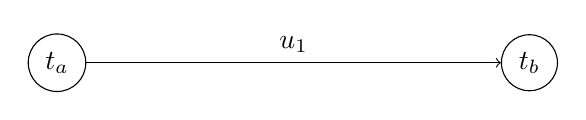
\begin{tikzpicture}
    \node[draw, circle] (ta) at (0,0) {$t_a$};
    \node[draw, circle] (tb) at (6,0) {$t_b$};
    \path [->] (ta) edge node[above] {$u_1$} (tb);
  \end{tikzpicture}
\end{center}

A matching of users who can satisfy each other is a vertex cycle. See the simplest case below:

\begin{center}
  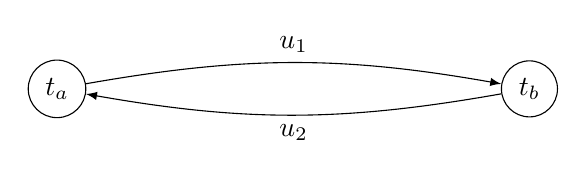
\begin{tikzpicture}
    \node[draw, circle] (ta) at (0,0) {$t_a$};
    \node[draw, circle] (tb) at (6,0) {$t_b$};
    \draw[-latex] (ta) to[bend left=10] node[above] {$u_1$} (tb);
    \draw[-latex] (tb) to[bend left=10] node[below] {$u_2$ }(ta);
  \end{tikzpicture}
\end{center}

The cycle packing problem \cite{Kri} characterises the goal of the matcher: find as many cycles with distinct edges (offer-request pairs). This problem is NP-Hard, although \cite{Kri} has an $\bO(\sqrt{\log n})$-approximation algorithm for it. I'm not yet clear whether the algorithm works with multiple edges between two nodes.

The matching problem can also be stated in terms of Weighted Boolean Optimization, a form of Integer Programming. Some additional features may be easier to add in this case, which is a common, reliable choice in the field despite being NP-complete.

The problem has been extensively studied for kidney exchanges \cite{Bir}, a sub-class of the offer network problem. In the kidney exchange problem, one has incompatible patient-donor pairs to be matched. This can easily be mapped into the offer network framework as: (offer=donor, request=patient). Kidney exchange networks tend to be thick (as there are only blood-types), and there is strong pressure to find exact algorithms for optimal matches as any sub-optimal match allows more patients to die.

An algorithm to find perfect weighted matchings in bipartite graph can be used to discover the optimal match in polynomial time \cite{Bir}. The bipartite graph has one side for Offers and one for Requests, thus each (offer=$t_a$, request=$t_b$) pair has two nodes created with edge weight $0$. Next an edge is created between the offfer node and every request node for $t_a$ with weight $> 0$. Then a maximum weight perfect matching algorithm can be used.

The drawback is that long-cycles are possible, and in the dense graph for kidney exchange, very likely. Each user reserves the right to refuse a suggested match, so longer matches are more likely to be rejected, and in the kidney case, require organizing dozens of simultaneous surgeries. However, bounding the match-size results in an NP-hard problem \cite{Bir}.

Below is a list of potentially desirable features that don't qualify for an MVP\footnote{minimal viable prototype}:
\begin{itemize}
  \item Reputation biased matching
  \item Preferences for matching based on
    \begin{itemize}
      \item User preferences
      \item Task prefreences
    \end{itemize}
  \item ORs and ANDs of offers or request
\end{itemize}


\end{document}
